%%
%%
%% This file should be edited by user
%%

\chapter{MicroC/OS-II} \label{chapter:osII}

To emphasize the characteristics of tinyOS, another OS, called OS-II, is presented. 
The MicroC kernel was developed by Jean J. Labrosse.

\section{Basics}

uC/OS-II is a portable, ROMable, scalable preemptive real-time multitasking kernel, written in ANSI-C. Small portions of the sourcecode are written in assembler to adapt to different processor architectures. uC/OS-II is based on uC/OS, also called \textit{The Real Time Kernel}, which was published in 1992. uC/OS v1.11 is compatible to its successor.

uC/OS-II is used in all kinds of embedded systems, ranging from engine controls to audio equiment.

\subsection{Main Features}

Important characteristics of this real-time multitasking OS are:

\begin{itemize}
 \item Scaleable, with a minimum RAM footprint of 6KByte
 \item Maximum RAM footprint 24KByte
 \item Preemptive Scheduler
 \item 10 Kernel Services
 \item 80 System Calls
 \item Support for semaphores
 \item Support for event flags
 \item Support for Message Queues
 \item Support for Message Mailboxes
 \item Up to 250 Application Tasks
 \item Constant / Deterministic execution time for most services provided
 \item Support for large number of processor architectures
 \item Supported processors range from 8bit to 64 bit architectures
 \item Supports Multi-Threaded Applications 
\end{itemize}

\section{Differences tinyOS - MicroC/OS-II}

\subsection{Real-Time}

A real-time system is a system where not only the correctness of a calculation is important, but also the instant \textbf{when} this calculation was finished. The most import features of a real-time kernel are minimal and predictable interrupt latency and task switching latency.

While uC/OS-II supports a timely determinstic behaviour, no such assertion can be given for tinyOS.

\subsection{Scheduler}

MicroC/OS-II has a \textit{preemptive} scheduler - that means that every task gets only a limited time for using the CPU. The time a task gets for execution also depends on the task's \textit{priority} - all tasks \textbf{MUST} have different priorities, because otherwise additional round-robing scheduling or similar would be necessary to handle tasks with equal priority. More important tasks get higher priority.

A task can be in 5 different states, as shown in figure \ref{fig:tasksstates}:

\begin{figure}[h]
 \centerline{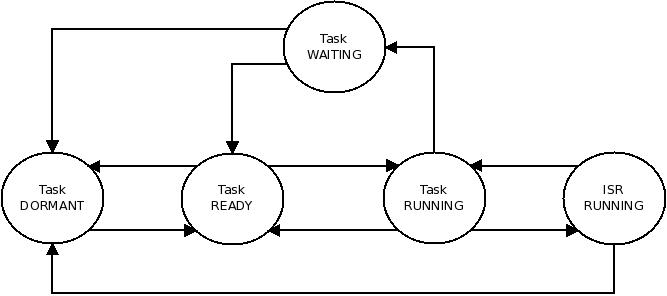
\includegraphics[width=.8\columnwidth]{pics/uCtasks.png}}
  \caption{Statemachine for Tasks}
  \label{fig:tasksstates}
\end{figure}

\begin{itemize}
 \item Dormant: task is loaded in memory but not ready to run yet
 \item Read: task is ready to run, but higher-priority task is running at the moment 
 \item Running: task is in control of the cpu
 \item ISR: interrupt has occured, cpu is executing ISR instead of task
 \item Waiting: task waits for an event(completion of IO operation, ...)
\end{itemize}

In contrast, tinyOS knows only 3 states:

\begin{itemize}
 \item Queued: task is queued, but sooner queued task is running at the moment 
 \item Running: task is in control of the cpu
 \item ISR: interrupt has occured, cpu is executing ISR instead of task
\end{itemize}

Also, as already said, tinyOS uses a non-preemptive scheduler, see chapter \ref{chapter:tinyos} for details.

\subsection{Mutual Exclusion}

Whenever different tasks need to share data with each other, some points must be ensured to avoid data corruption and resource contention. Problems arise, for example, if task A gets scheduled and accesses a dataelement that is also needed by task B. If task A gets preemted by task B before task's A calculations are finished, task B works on incomplete data, possibly invalidating it's own calculations. To prevent such situations, MicroC/OS-II provides the following mechanisms:

\begin{itemize}
 \item Disabling/Enabling of interrupts with macros 
 \item Semaphores
\end{itemize}

By \textit{disabling interrupts}, a task or ISR can assure that it won't get preempted by an ISR or by a task, so this is an easy way to grant mutual exclusion. Drawbacks of this solution are that the system obviously can't react to other - possibly important - interrupts. Additionally, because the Micro/OS-II kernel uses timeslicing, the task scheduler is deactivated because no timer interrupts are handled. So, a badly designed task can halt the whole system if it enters a deadlock or some kind of endless loop.

\textit{Semaphores}, developed by Edsger W. Dijkstra, are softwareconstructs that can be used for the same goal. Additionally, they can be used for syncronizing tasks, as described in the following section.

Because tinyOS uses a non-preemptive scheduler, no such constructs are neccessary. Because a task cannot get suspended, apart from an interrupt, by another task, every task is responsible to keep it's data in a consistent state.

\subsection{Intertask Communication}

The process of sharing data between different tasks or ISRs is called \textit{intertask communication}. Therefore, MicroC/OS-II supports the following ways of sharing data between tasks

\begin{itemize}
 \item Message Mailboxes
 \item Message Queues 
\end{itemize}

MircoC/OS-II provides kernel services to send messages by depositing a pointervariable into a task's mailbox. A task that expects such a message is supended and put onto a waitinglist. If the message arrives within a timeout, the highest-priority task that is waiting for the message is woken up.

A message queue is basically an array of such message mailboxes.

In tinyOS, a task can share data by passing a pointer to the datastructure used, or by using global variables.

\subsection{Task Syncronisation}

\begin{itemize}
 \item Semaphores 
 \item Event Flags
\end{itemize}

Aside from using semaphores for granting mutual exclusion, this software constructs can also be used to syncronize a task with an ISR or other tasks.
Additionally, MicroC/OS-II offers kernel services to \textit{set}, \textit{clear} and \textit{wait} for event flags.

Syncronisation in tinyOS is implemented by \textit{events}.

\subsection{Memory Footprint}

When using a kernel to manage tasks, the total memory that is needed consists of the application code size + the kernel code size. A minimum ram footprint of 6kByte is given by the developer of MicroC/OS-II.

In tinyOS, the ram needed for the kernel FIXME

\subsection{Supported Platforms}

%%
%% = eof =====================================================================
%%
